%\usepackage{pgf-umlsd}
\chapter{Netcode Mechaniken}
\label{Netcode}
Im folgenden Abschnitt werden die im Projekt umgesetzten und verwendeten Mechaniken beschrieben.
Hierbei liegt der Fokus darauf, ein durchdachtes System zu verwenden, das den Kern der Problematik einfach im Spiel erkenntlich machen kann. 
Viele der Mechaniken ergänzen sich gegenseitig und sind somit auch eng miteinander verbunden in der Implementierung als auch von der theoretischen Definition.
(Mögliche Referenz zum Grundlagenteil)

In der Fachliteratur und technischen Dokumentation finden sich unterschiedliche Auffassungen zur Einordnung zentraler Netcode-Mechanismen wie Client-Side Prediction, Reconciliation, Lag Compensation und Interpolation. Zwei grundlegende Perspektiven lassen sich dabei unterscheiden:


\textbf{Funktionale Trennung:} In dieser Sichtweise werden die Mechanismen entlang ihrer funktionalen und systemarchitektonischen Zuständigkeit voneinander abgegrenzt. Lag Compensation wird dabei als rein serverseitige Rückrechnung von Spielzuständen verstanden, während Prediction und Reconciliation auf Client-Seite zur Vorhersage und Korrektur genutzt werden. Interpolation dient primär der visuellen Glättung gegnerischer Bewegungen und wird als unabhängige Darstellungsmechanik betrachtet. Diese Perspektive wird unter anderem von Glenn Fiedler \cite{fiedlerPrediction} vertreten. \newpage
    
\textbf{Systemische Integration:} In der erweiterten Lesart – wie sie beispielsweise von Valve in der Dokumentation zur Source-Engine \cite{valveLagComp} vertreten wird – wird Lag Compensation als Sammelbegriff für alle Verfahren verstanden, die zur Kompensation von Netzwerklatenz und Synchronisationsabweichungen beitragen. Hier sind Prediction, Reconciliation und Interpolation funktional stark miteinander verknüpft und technisch teils gemeinsam implementiert, etwa durch geteilte Zustands- und Eingabepuffer.


Beide Sichtweisen bieten wertvolle Konzepte für den Entwurf und das Verständnis verteilter Spielsysteme. Im Folgenden wird gezeigt, wie diese Ansätze in der vorliegenden Arbeit kombiniert und auf ein praktisches Prototypsystem übertragen werden.
Im Rahmen dieses Projektes wird ein System verwendet, das die Bewegungs und Schussmechanik trennt, wobei innerhalb der Bewegungsmechanik Lag Compensation und Client Side Prediction eng miteinander verbunden sind. Dies hat wie in \autoref{Netzwerkarchitektur} bereits angerissen, den Vorteil, dass das für das Target verwendete System, somit keinen systematischen Austausch zwischen Client(s) und Server benötigt.
Dies spart semantische als auch syntaktische Komplexität, die bei einer kompletten systematischen Integration nur schwer verständlich wäre. 

\begin{figure}[H] % oder [htbp]
    \centering
    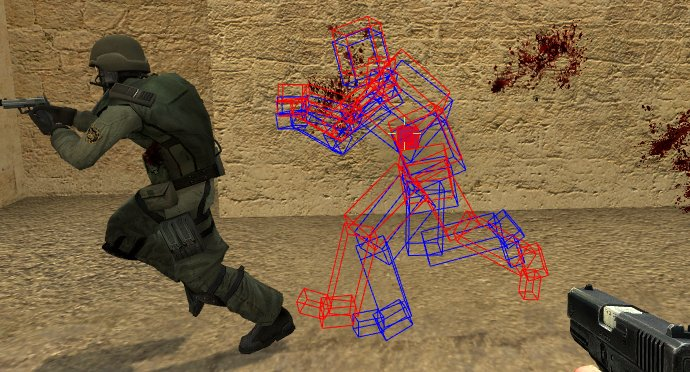
\includegraphics[width=0.8\textwidth]{figures/lag_comp_valve.png}
    \caption{lag comp source engine}
    \label{fig:lag comp}
\end{figure}


\section{Client-side Prediction beim Bewegen und Schießen}
\label{client side prediction}

In einem serverautoritativen Netzwerkmodell ist es essenziell, ein faires und sicheres Spielumfeld zu gewährleisten. Gleichzeitig darf die Spielbarkeit aus Sicht des Spielers nicht unter einer hohen Latenz leiden. Besonders bei reaktionsintensiven Genres wie First-Person-Shootern oder Rennspielen ist eine direkte Rückmeldung auf Eingaben entscheidend für das Spielerlebnis.

Ein vollständiger Verzicht auf Client-Authorität würde zwar maximale Sicherheit bieten, jedoch zu spürbarer Verzögerung bei der Bewegung oder Aktion führen. Ziel ist daher ein Kompromiss: Der Server behält die Entscheidungsgewalt, während der Client Eingaben sofort lokal umsetzt und visuelles Feedback liefert.

Bei der Visualiersierung sind in diesem Bereich keine ausschlaggebenden Erkenntnisse zu ziehen. Es handelt sich hierbei am ehesten um eine reine Feedback-Mechanik, die höchstens kumulativ in die Diskrepanz der eigentlichen Position des Clients und der vom Server gehaltene Position des Clients mit einfließt. 


\newpage
In der vorliegenden Implementierung wird dies durch ein Überschreiben der Unity-eigenen \texttt{NetworkTransform}-Komponente realisiert. Die Autoritätslogik wird über eine einfache Enumeration gesteuert:

\lstinputlisting[
  style=csharpStyle,
  caption={Überschreiben der NetworkTransform-Komponente mit AuthorityMode},
  label={lst:authority-mode} 
]{src/PlayerMovement/ClientNetworkTransform.cs}


Die Methode \texttt{OnIsServerAuthoritative()} gibt in der Regel \texttt{false} zurück, sodass der Client die Kontrolle über Bewegung und Eingabe erhält, ohne dass ein Roundtrip zum Server erforderlich ist. Dadurch wird die Latenzwahrnehmung(Ping), beim Spieler erheblich reduziert.

\newpage
\section{Reconciliation – Zustandskorrektur  bei Abweichungen}

Trotz lokaler Vorhersage durch den Client bleibt der Server die Referenzinstanz für den „wahren“ Spielzustand. Sollte es zu größeren Abweichungen zwischen Client- und Serverposition kommen, wird ein Reconciliation-Prozess ausgelöst. Dabei wird der Client zurück auf den zuletzt vom Server bestätigten Zustand gesetzt und die eigenen Eingaben ab diesem Zeitpunkt erneut simuliert.

In Spielen mit präzisem Bewegungsfeedback (z.B. FPS) ist die Toleranzschwelle für Positionsfehler oft sehr gering. In diesem Projekt wurde ein Grenzwert: \\ (\texttt{reconciliationThreshold}) definiert, ab dem eine Zustandskorrektur erfolgt. Dieser Wert kann abhängig von variabler Netzwerklatenz angepasst werden.
\begin{figure}[h] 
  \centering
  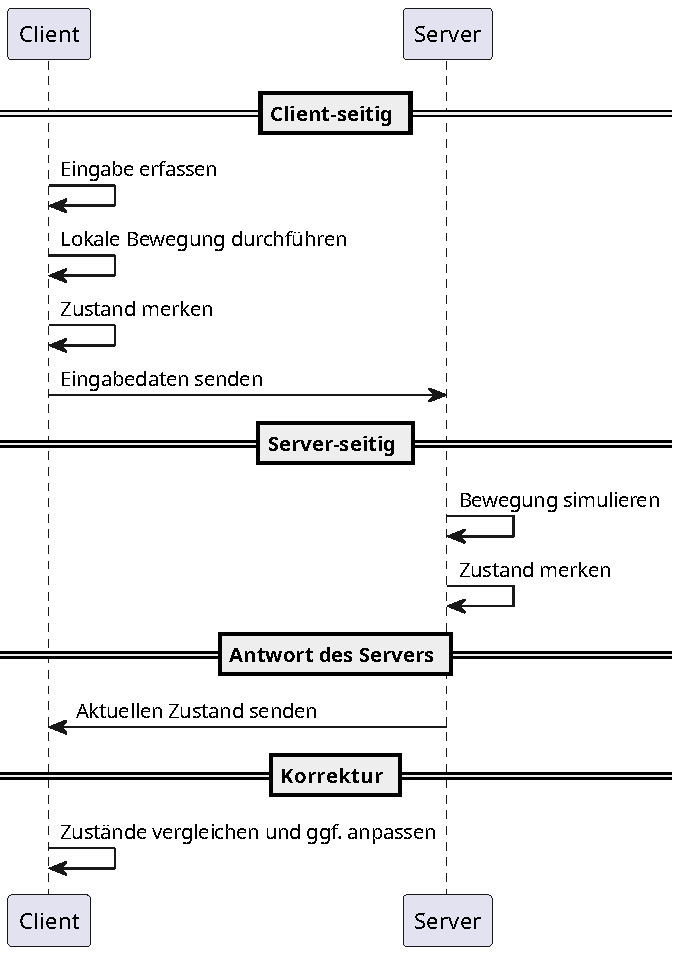
\includegraphics[width=0.4\textwidth, keepaspectratio]{out/diagrams/Reconciliation-high/Reconciliation-high.pdf} %Größe ist noch ausbaufähig...
  \caption{High Level Ablauf der Reconciliation }
  \label{fig:rec}
\end{figure}

\newpage
\section{Testmechanismus zur Validierung}
\label{Reconciliation-Test}

Zur gezielten Auslösung der Reconciliation wurde ein einfacher Testmechanismus implementiert: Ein Client-Cheat teleportiert den Spieler um 20 Einheiten nach vorne – weit über die Fehlertoleranz hinaus. Der Server erkennt die Abweichung und triggert die Korrektur, wodurch der Spieler sichtbar in den korrekten Zustand „zurückspringt“.

Zur Visualisierung wurden farblich unterschiedliche Proxies über dem Spielerobjekt angezeigt, die die vom Client bzw. Server berechneten Zustände darstellen. Wenn somit künstlich hinzugefügte oder native Latenz dazukommt, soll sich bei Bewegung der Abstand der Proxies vergrößern.
Diese Proxies sind intern als einfache 3D-Objekte im Unity Editor als Prefabs angelegt worden. Sie eignen sich hierbei als Sphären oder Kugeln, da man so einfachste Positionsunterschiede leicht erkennen kann. 

In der Praxis wird dies mit einem kleinen Cheat implementiert, welcher sich in Form eines Teleport-Taste äußert. Wenn diese Taste gedrückt wird springt der Spieler inklusive des Client Proxy nach vorne also um 20 Einheiten in Z-Richtung.
Wenn somit der Client inklusive Proxy die Schwelle überschritten haben signalisiert das dem Server, dass eine ungültige Aktion geschehen ist und setzt den Spieler auf seine letzte gültige Position, Geschwindigkeit und Rotation zurück.
Da dies in Echtzeit ziemlich schnell passiert kann man mit einem \texttt{Debug.Break()} den Frame einfrieren an dem die Schwellenüberschreitung geschehen ist, was in folgender Abbildung erkenntlich ist.
%\includegraphics{}
Man sieht hier also genau diese Teleportierung die unter umständen von Spielern ausgenutzt werden könnte, sollte keine sinnvolle Reconciliation exisitieren. Je nach Spiel ist somit eine sinnvolle Schwelle zu wählen, die unter umständen auch variabel ist und sich an Netzwerkkonditionen anpasst.
In Taktischen Shootern bswp. wäre ein grundsätzlicher Ansatz sinnvoll, die Schwelle etwas niedriger zu halten und bei hohem Ping des Spielers diese Schwelle variabel zu erhöhen. Dieser Ansatz ist vor allem dann sinnvoll wenn vom Spielentwickler viel Wert auf Präzision gelegt wird. Ein sinnvoller Grundwert würde hier zwischen 5-10 Einheiten liegen. In diesem Szenario ist alles legitim was unter dem Wert der Teleport-Distanz liegt und wird dann im späteren Ablauf auf die schlechter werdenden Netzwerkkondition angepasst beziehungsweise erhöht.

\section{Datenstrukturen und Ticksystem}
Als Datenstruktur wurde für das Ticksystem auf einen Ringpuffer gesetzt. Im Netcode-Bereich ist dies defacto Standard <Quelle maybe> um die mit den einzelnen Ticks verbundenen Informationen oder genauer Positionen, Rotationen und Geschwindigkeiten umzugehen und Overheads zu negieren. 
Demnach eignen sich bspw. Arrays oder Dictionaries deutlich schlechter, da diese die gespeicherten Informationen nicht verwerfen und somit unnötige Daten halten, die für bspw. die Reconciliation außer Reichweite liegen und somit die Performance beeinträchtigen.
In Kombination mit State und Input Payloads die jeweils als Structs implementiert wurden, sollen die Positionen zum passenden Tick verglichen werden können.
Die Eigenimplementierung des Ringpuffers ist somit generisch und basiert auf den Input oder State Payloads. Mit der Methode Add(), die ein generisches Item also in diesem Fall das State oder Input Payload und einen Index als Parameter nimmt, kann somit der Puffer befüllt werden.
Das Befüllen folgt den algorithmischen Grundlagen eines solchen Buffers und das geschieht bis zu der statischen Buffergröße und fängt dann wieder von null an zu indezieren. 
Somit werden in diesem Fall intern bis 1024 Ticks verwaltet, was bei einer Standard-Tickrate von 60Hz ungefähr 17 Sekunden wären, die man zurückspulen könnte. 
Eine solche Puffergröße ist großzügig, sollte man jedoch auf eine Tickbasis aufsteigen von etwa 128Hz, ist die mögliche Rückspulzeit somit schon sinnvoller. In Anwendungsfällen ist ein Rückspulen was über eine Sekunde her ist spielhindernd und würde die Spielererfahrung deutlich verschlechtern. 

\newpage

In der Abbildung \ref{lst:circular-buffer} sieht man noch den Aufbau des Circular Buffers und die Strukturen die essentiell sind für den Datentransfer:
\lstinputlisting[
  style=csharpStyle,
  caption={Methode \texttt{CircularBuffer()}},
  label={lst:circular-buffer}
]{src/CircularBuffer.cs}

\newpage
Auf der anderen Seite muss dies durch die angesprochenen Strukturen gespeichert werden:
\lstinputlisting[
  style=csharpStyle,
  caption={Methode \texttt{Payload}},
  label={lst:payload}
]{src/Payload.cs}
In der InputPayload werden die Eingabedaten des Spielers verwaltet und serialisiert, was über die vom zu implementierenden Interface INetworkSerializeable gestellten Methode NetworkSerialize() getan wird.

\section{Kernmethoden der Reconciliation-Logik}
Im Grunde lässt sich die Logik auf einige Methoden runterbrechen, dies sich alle im PlayerMovement Skript befinden. Diese Methoden sind jedoch verschachtelt in einem komplexeren Ablauf dieses Skriptes, reichen aber fürs Verständnis aus. 
\newpage
\begin{enumerate}
    \item \texttt{ShouldReconcile()} \\
    Diese Methode prüft, ob neue Serverdaten vorliegen und ob diese sich vom zuletzt verarbeiteten Zustand unterscheiden:

\lstinputlisting[
  style=csharpStyle,
  caption={Methode \texttt{ShouldReconcile()}},
  label={lst:should-reconcile}
]{src/PlayerMovement/ShouldReconcile.cs}

    \item \texttt{ReconcileState(StatePayload rewindState)} \\
    Hier wird der Client-Zustand auf den vom Server bestätigten Zustand zurückgesetzt. Anschließend werden alle seitdem aufgezeichneten Eingaben erneut angewendet:

\lstinputlisting[
  style=csharpStyle,
  caption={Methode \texttt{ReconcileState(StatePayload)}},
  label={lst:reconcile-state}
]{src/PlayerMovement/ReconcileState.cs}

    \item \texttt{HandleServerReconciliation()} \\
    Diese Methode koordiniert den gesamten Reconciliation-Prozess und vergleicht die Zustände beider Seiten:

\lstinputlisting[
  style=csharpStyle,
  caption={Methode \texttt{HandleServerReconciliation()}},
  label={lst:handle-server-reconciliation}
]{src/PlayerMovement/HandleServerReconciliation.cs}

Wenn diese Prozesskette dann ausgeschlagen ist, wird in einer Methode die sich um die Tickverarbeitung beim Client kümmert, aufgerufen.
Diese Methode: \texttt{HandleClientTick()} soll also nur aufgerufen werden, wenn es sich bei der aktuellen Instanz um einen Spieler handelt. Hier wird mit den vom NetworkBehaviour geerbten Eigenschaften:
\begin{itemize}
  \item \texttt{!IsClient}
  \item \texttt{!IsOwner}
\end{itemize} 
geprüft ob es sich wirklich um einen Spieler und nicht doch eine Serverinstanz handelt. 
Sollte dies jedoch nicht der Fall sein, wird die Methode verlassen und die analog aufgebaute Methode zur Server-Tickverarbeitung aufgerufen: \texttt{HandleServerTick()}.

Zusätzlich ist wichtig, dass der Spieler bei häufiger Desynchronisation über dem erlaubtem Limit häufig zurückspringt. Das kann man auf verschiedene Weisen unterbinden, allerdings haben diese Herangehensweisen auch oft Nachteile. 
Hierbei ist ein Cooldown implementiert, der eine wiederholte Reconciliation zeitlich beschränkt. Nach jeder Reconciliation läuft somit ein Cooldown-Timer und erst nach Ablauf davon, kann der Spieler manuell oder durch zu hohen Desync zurückgesetzt werden. 
Wie bereits angesprochen hat das auch Nachteile und Risiken und somit muss in echten Szenarien ein Missbrauch dieser Mechanik unterbunden werden. Wenn ein Spieler über einen Cheat verfügt, ähnlich wie der in \ref{Reconciliation-Test} Testmechanismus, jedoch extern und ungewollt.
\section{Lag Compensation für Bewegung}

Mit Lag Compensation wird versucht schlechte Netzwerkkonditionen auszugleichen. Wenn also ein Client eine unstabile Verbindung zum Server hat, soll Lag Compensation einen approximativen Ausgleich schaffen im besten Fall ohne, dass einer der Clients im Vorteil ist.
Hierbei werden bei einer lokalen Testumgebung in Unity künstliche Latenzen, Paketverlust oder Jitter eingefügt um besagte Netzwerkkonditionen zu replizieren.
Das beschriebene System für Lag Compensation bezieht sich auf die Spielerbewegung und ist somit eng mit dem System der zuvor angesprochenen Reconciliation verbunden, demnach ist auch das Validierungsumfeld sehr ähnlich.
Technisch gesehen, ist Lag Compensation die Obermenge von allen Werkzeugen, die das Verstecken von Latenz oder ungünstigen Netzwerkkonditionen berwerkstelligen sollen. 
Dennoch lässt sich Lag Compensation explizit mit einer häufig verwendeten Mechanik, nämlich der Extrapolation implementieren. Extrapolation ist eine gängige Form, Netcode Szenarien, bei fehlenden Serverupdates zu bewältigen. Hierbei ist es wichtig abzuwägen und auch einzuordnen, ob der Client überhaupt noch Updates an den Server sendet oder schon von einem Verbindungsabbruch des Clients die Rede ist.
In diesem Zeitraum jedoch soll geschätzt werden, anhand der letzten bekannten Eingabewerte, wo sich der Client als nächstes befinden wird.
(Hier der stuff mit Unity am besten...) => wahrscheinlich bessere und ausführlichere Erkläreung... 

alternativ:
Lag Compensation bezeichnet eine Gruppe von Verfahren zur Abmilderung negativer Effekte instabiler Netzwerkverbindungen, insbesondere erhöhter Latenz, Paketverlust und Jitter. Ziel dieser Mechanismen ist es, trotz solcher Störungen eine möglichst kohärente und faire Spielerfahrung sicherzustellen – idealerweise ohne spürbare Vor- oder Nachteile für einzelne Clients.
Die vorliegende Arbeit fokussiert sich auf Lag Compensation im Kontext der Bewegungssynchronisation. Eine klare Abgrenzung ist dabei zur Lag Compensation bei Treffererkennung (z.B. rückwirkende Hit-Prüfung bei Schusswaffen) erforderlich, wie sie insbesondere in kompetitiven Shootern zum Einsatz kommt. Während dort meist serverseitige Backtracking-Verfahren genutzt werden, steht hier die clientseitige Kompensation von Bewegungslatenz im Vordergrund.
Zur Untersuchung der Mechanismen wurde eine lokale Testumgebung in Unity entwickelt, in der sich Netzwerkanomalien wie Latenz, Paketverlust und Jitter gezielt simulieren lassen. Diese bildet die Grundlage für die Validierung verschiedener Kompensationsstrategien.
Technisch lässt sich Lag Compensation als Oberbegriff für sämtliche Verfahren verstehen, die Zustandsverzögerungen kaschieren oder korrigieren – darunter Client-Side Prediction, Reconciliation, Interpolation und Extrapolation. Im Kontext der Bewegungssynchronisation kommt insbesondere Extrapolation zum Einsatz, also die Vorwärtsschätzung eines Objektzustands bei verzögerten oder ausbleibenden Serverupdates.
Hierbei wird – basierend auf den zuletzt bekannten Zuständen wie Position, Rotation und Geschwindigkeit – eine plausible Fortsetzung der Bewegung berechnet. Dies erlaubt es, Objekte auf dem Client weiterhin konsistent darzustellen, obwohl keine aktuellen Daten vom Server vorliegen. Gleichzeitig muss jedoch berücksichtigt werden, ob tatsächlich nur temporär keine Updates empfangen werden oder ob bereits ein dauerhafter Verbindungsabbruch vorliegt, da sich daraus unterschiedliche Handlungsstrategien ergeben.
Das in Unity implementierte System nutzt daher eine Kombination aus Latenzerkennung, Timeout-Steuerung und extrapolierender Bewegungsschätzung, um unter kontrollierten Störbedingungen möglichst flüssige Bewegungsdarstellungen zu ermöglichen.

\section{Funktionsweise der Extrapolation}
Ob überhaupt extrapoliert werden soll, also ob überhaupt eine Rekonstruktion stattfinden soll, wird analog zur Reconciliation in einer Methode: \texttt{ShouldExtrapolate()} beurteilt.
Die Bedingung ist hierbei, ob die Latenz der aktuellsten Payload kleiner als das definierte Latenzlimit in Millisekunden ist, während sie gleichzeitig größer als das Zeitintervall der physikalischen Aktualisierungsfrequenz (FixedUpdate) ist, sodass eine Extrapolation notwendig und zugleich noch sinnvoll durchführbar erscheint. Sinnvoll ist eine Extraploation genau dann, wenn die Latenz des Spielers in einem Bereich von ungefähr 3-500ms liegt. In diesem Intervall kann man also von einem Client ausgehen, der unter normalen Konditionen mit dem Server verbunden ist.

hier könnte der code sein:

Ähnlich wie im Fall der Reconciliation wird auch bei der Extrapolation ein Cooldown-Timer verwendet. Dieser sorgt dafür, dass bei ausbleibenden Eingaben des Clients – etwa infolge von Paketverlust oder temporärer Verbindungsinstabilität – weiterhin eine plausible Vorwärtsschätzung der Bewegung vorgenommen wird. Der Zeitraum der Extrapolation ist dabei auf maximal fünf Sekunden begrenzt.

Die Einführung eines Timers bietet mehrere Vorteile: Zum einen kann mit einer konstanten angenommenen Latenz extrapoliert werden, was zu einer stabileren und nachvollziehbareren Bewegungsschätzung führt. Zum anderen wird vermieden, dass bei längerer Unterbrechung der Verbindung unkontrolliert oder unplausibel extrapoliert wird.

Gleichwohl stellt die Wahl der Extrapolationsdauer einen Kompromiss dar. Zu kurze Zeitfenster führen dazu, dass kurzfristige Aussetzer nicht abgefangen werden, während zu lange Zeiträume die Gefahr von Positionsabweichungen erhöhen. Im Idealfall müsste die zulässige Extrapolationsdauer adaptiv an die konkreten Netzwerkverhältnisse des jeweiligen Clients angepasst werden.

Obwohl eine adaptive Anpassung der Extrapolationsdauer an individuelle Netzwerkbedingungen denkbar wäre, hat sich in der Praxis die Verwendung eines festen Grenzwerts als robuster und konsistenter erwiesen. Eine dynamische Lösung würde zusätzlichen Overhead erzeugen, ohne signifikante Vorteile in der Bewegungsgenauigkeit zu garantieren.


\newpage

\section{Datenstrukturen}
Als Datenstruktur wird der bereits bestehende StatePayload verwendet und jedlglich um ein neues Feld von diesem Typen ergänzt. Zusätzlich wird auf das in \ref{client side prediction} angepasste (Klasse) ClientNetworkTransform-Modell für die Authoritätenänderung zugegriffen. Diese Komponente wird benötigt um während der Extrapolation variabel die Authoriät zu ändern.

\subsection{Timer}
Spezifisch werden für die Extrapolation CountdownTimer verwendet die inklusive Events, die diesen Ablauf regulieren, in einem ausgelaberten Hilfs-Namespace zu finden. Dieser Ablauf wird in der Unity Hook Awake gesteuert.

\section{Datenstrukturenrr}
Für die Extrapolation wird die bestehende Datenstruktur \texttt{StatePayload} verwendet, die um ein zusätzliches Feld zur Speicherung des extrapolierten Zustands erweitert wird. Darüber hinaus greift das System auf die in \ref{client side prediction} beschriebene Klasse \texttt{ClientNetworkTransform} zurück, welche in modifizierter Form eingesetzt wird, um eine dynamische Änderung der Autorität während der Extrapolation zu ermöglichen.

\subsection{Timerrr}
Zur Steuerung der Extrapolation werden spezielle \texttt{CountdownTimer}-Instanzen verwendet, die im Rahmen eines Hilfs-Namespaces implementiert sind. Diese Timer unterstützen Events zur gezielten Regelung des Ablaufs. Die Initialisierung erfolgt in der Unity-Hook \texttt{Awake}.

\section{Kernmethoden der Extrapolation}
Da Extrapolation eine serverseitige Mechanik ist, muss eine Prüfung stattfinden, welche Instanz gerade die Eingabebearbeitung ausführt.
Nur in genau dem Fall, dass die Verabeitung vom Server vom Host durchgeführt wird und der Cooldown für die Extrapolation gerade am laufen ist, wird also die Methode \texttt{Extrapolate()} aufgerufen.

In dieser Methode wird die Position des Transforms des Character Controllers auf die zuvor berechnete Position aus der Extrapolation-Payload gesetzt. Dabei wird die Y-Koordinate explizit auf null gesetzt, um vertikale Bewegungen – etwa durch physikalische Effekte oder fehlerhafte Schätzungen – auszuschließen und eine stabile Bewegung ausschließlich in der XZ-Ebene sicherzustellen.
Dieser beschriebene Ablauf wird mit 2 Methoden bewältigt:

\lstinputlisting[
  style=csharpStyle,
  caption={Extrapolation},
  label={lst:extrapolation}
]{src/PlayerMovement/Extrapolation.cs}

\newpage

\textbf{Extrapolationsvektor (posAdjustment)}

Zur Schätzung einer zukünftigen Position bei fehlenden Netzwerkupdates wird die zuletzt bekannte Geschwindigkeit $\vec{v}$ mit einer gewichteten Zeitkomponente multipliziert. Diese ergibt sich aus der gemessenen Latenz $\lambda$ und einem anpassbaren Multiplikator $\alpha$ zur Feinsteuerung der Extrapolation:

\[
\vec{d} = \vec{v} \cdot \left(1 + \lambda \cdot \alpha\right)
\]

Dabei ist:
\begin{itemize}
    \item $\vec{d}$ der extrapolierte Bewegungsvektor (engl. \textit{posAdjustment}),
    \item $\vec{v}$ die letzte bekannte Geschwindigkeit des Objekts,
    \item $\lambda$ die Latenzzeit in Sekunden,
    \item $\alpha$ ein konfigurierbarer Multiplikator (typischerweise $\alpha = 1.2$).
\end{itemize}

Die so berechnete Bewegung wird zur letzten bekannten Position $\vec{p}_\text{alt}$ addiert, um die extrapolierte Zielposition $\vec{p}_\text{neu}$ zu erhalten:

\[
\vec{p}_\text{neu} = \vec{p}_\text{alt} + \vec{d}
\]

\textbf{Beispiel}

Gegeben sei eine Geschwindigkeit $\vec{v} = (2, 0, 1)$ in Metern pro Sekunde, eine Latenz von $\lambda = 0{,}3$ Sekunden sowie $\alpha = 1{,}0$. Daraus ergibt sich:

\[
\vec{d} = (2, 0, 1) \cdot (1 + 0{,}3 \cdot 1{,}0) = (2, 0, 1) \cdot 1{,}3 = (2{,}6, 0, 1{,}3)
\]

Die Position des Objekts kann damit während einer Netzwerkunterbrechung um ca. $2{,}6\,\text{m}$ in $x$- und $1{,}3\,\text{m}$ in $z$-Richtung extrapoliert werden.

\newpage

Mit der gegebenen Latenz wird entweder für die volle Zeitspanne des Cooldown Timers extrapoliert, oder es wird abgebrochen, falls die Latenz über oder unterhalb der Schwellen liegt.

\section{Lag Compensation beim Schießen}
Als Basis für die Implementierung der Lag Compensation im Kontext der Treffererkennung wird ein separates System genutzt, das sich von jenem zur Spielerbewegung unterscheidet. Theoretisch wäre es möglich, sowohl die Bewegung als auch die Schussmechanik in einem gemeinsamen Modul — etwa innerhalb eines übergreifenden \texttt{PlayerController}-Skripts — zu integrieren, welches weiterhin auf dem bereits etablierten Payload-System basiert. Diese Koppelung wurde jedoch, wie bereits in Abschnitt~ \ref{client side prediction} erläutert, bewusst vermieden.
Stattdessen wird auf einem dedizierten \texttt{Gun}-Skript aufgebaut, das für die grundlegende Waffenlogik, Treffererkennung, sowie die clientseitige Wiedergabe von Waffenanimationen und Audiosignalen zuständig ist.
Im Vergleich zur Bewegungsmechanik erscheint die technische Umsetzung hier zunächst einfacher. In einem vollständig einsatzfähigen Mehrspieler FPS-System ist jedoch das Gegenteil der Fall: Die Korrektheit der Trefferregistrierung ist ein zentrales Element für das Spielgefühl. Besonders in Verbindung mit Lag Compensation stellt diese Komponente eine erhebliche Herausforderung dar. In realistischen Netzwerkumgebungen gibt es zahlreiche Randbedingungen und Einflussgrößen, die nicht ohne weiteres in ein allgemeingültiges System integriert werden können, ohne erhebliche Performanceeinbußen zu riskieren.

In älteren Titeln wie \textit{Quake} oder \textit{Doom} war die Entscheidung, ob überhaupt eine Lag Compensation implementiert wird, ein wesentlicher Bestandteil des Spieldesigns — eine Option, die in modernen Spielen kaum mehr denkbar ist. Gerade in Shootern stellt Lag Compensation heute ein zentrales Mittel dar, um ungleiche Netzwerkverhältnisse zwischen Clients bestmöglich auszugleichen.
Ohne entsprechende Kompensation wären Spieler mit hoher Latenz insbesondere in Bewegung nur schwer bis gar nicht zuverlässig zu treffen, da die Differenz zwischen dem serverseitigen Zustand und dem, was der Client darstellt, zu groß wird. Dies führt zu einer teils erheblichen Verschiebung der effektiven Hitbox und damit zu unnatürlichen Spielerlebnissen.
\newpage

Der Grundsätzliche Ablauf lässt sich wie folgt ableiten:
\begin{figure}[h] 
  \centering
  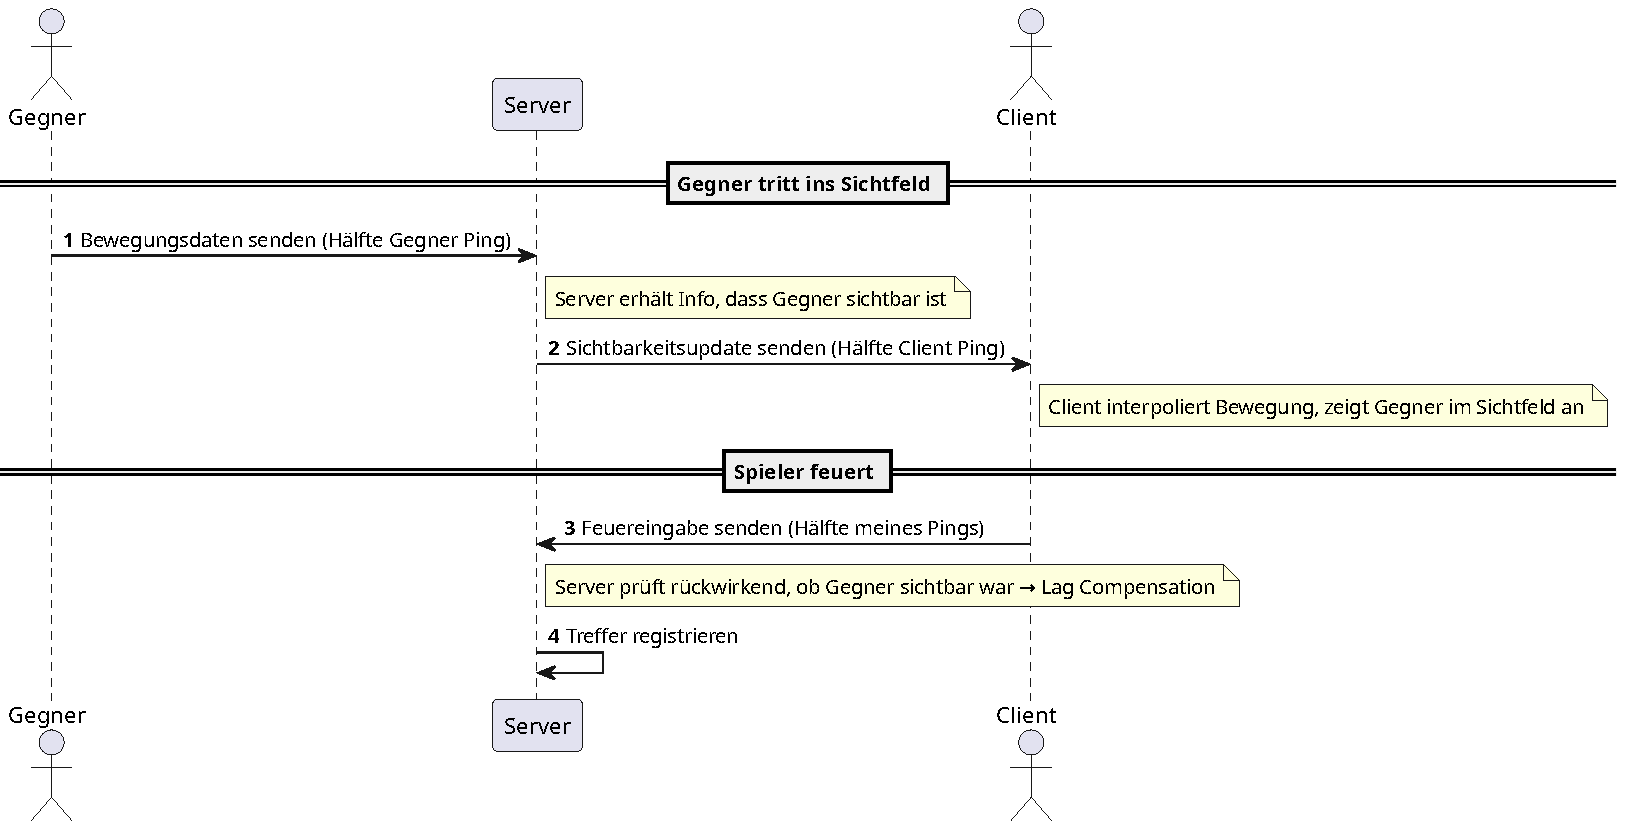
\includegraphics[width=0.9\textwidth, keepaspectratio]{out/diagrams/lag-comp-csgo/lag-comp-csgo.pdf} %Größe ist noch ausbaufähig...
  \caption{Visualisierung der Lag Compensation}
  \label{fig:shhhhshshs}
\end{figure}

Mit dieser Mechanik lässt sich zwar kein sauberes Spielgefühl erzeugen und sorgt immernoch nicht für ein faires Spielverhältnis wenn die involvierten Spieler nicht ähnlich hohe Latenzen haben.
Jedoch ist dieses Verfahren das weitverbreiteste in der Branche, was bislang noch keinen würdigen Nachffolger erhalten hat, der die durch Lag Compensation entstandenen Probleme löst.
Die klassischen Probleme sind hierbei:
\begin{itemize}
  \item Auf einen Client registrieren Treffer, obwohl er in Deckung ist
  \item Gegner registriert Schüsse auf einen Client obwohl er für den Client nicht sichbar ist
  \item Peeker's Advantage
  \item Killtrades
\end{itemize}

Die beschriebene Problematik ist nicht immer vollständig auf Lag Compensation zurückzuführen, jedoch bevorzugt sie in den meisten Fällen den Spieler mit dem geringeren Ping.
In einem Szenario, in dem beide Spieler bspw. gleichzeitig aufeinander schießen und treffen würden -- was im Kontext von Netcode nahezu paradox ist -- würde allerdings die Bestätigung für den Treffer oder Abschuss, den Spieler mit dem geringeren Ping früher erreichen.
Das wäre für die meisten Entwickler kein ideales aber dennoch faires Szenario, denn ein niedriger Ping sollte zumindest keinen Nachteil einbingen. In manchen Fällen und Spielen wird hierfür überkompensiert, sodass höherer Ping im Bereich von 60-80ms vorteilhaft ist -- vor allem beim Initiieren eines Duels (peeking). In dieser Implementierung, wie es bei Valorant der Fall ist, muss auf bestimmte Ping-Bereiche eingegangen sein und mit variablen Multiplikatoren gearbeitet worden sein, um somit für die meisten Szenarien diesen Vorteil (Peeker's Advantage) zu minimieren \cite{valorantPeeker}. 
Es gibt somit keinen Idealzustand für eine Integration von beliebten Netcode-Mechaniken, die für direkte Client-Eingabe sorgen und gleichzeitig ein zeitlich faires und korrektes System stellen. 

% Hier ziemlich sicher Redundanz mal aufpassen
Im Rahmen der Arbeit wird jedlglich versucht diese Problematik zu visualisieren, da die Grundlage eine andere ist. In einem Szenario in dem es nur einen Spieler und ein vom Server gesteuertes Zielobjekt gibt, ist die Komplexität und Signifikanz der Lag Compensation geringer.
In diesem Fall kann also keine vollständige Implementierung von einer Treffererkennung und Lag Compensation gezeigt werden wie sie in PvP-Spielen vorkommt, allerdings wird ein Modell gezeigt, dass versucht diesen Sachverhalt unter den genannten Einschränkungen zu veranschaulichen. 


\subsection{Aufbau der Replikation}
Um in Unity Lag Compensation beim Schießen darzustellen, ist ein bewegliches Ziel im Einsatz, welches intern wieder ein 3D-Objekt (Sphere) als sogenanntes Enemy-Prefab eingebunden ist. Das Prefab ist außerdem ein Network Objekt, allerdings ohne eines Network Transfomrs für die Synchronisation, welche in diesem Kontext selbstständig implementiert ist. Dieses Ziel soll die horrizontale Bewegung eines echten Spielers replizieren, allerdings über den Server gesteuert. Das bedeutet wiederum, dass das zuständige Target-Skript nur auf dem Server ausgeführt werden darf und wird.
(hier noch überlegen, ob das Base-Skript wo anders erklärt werden soll).
Somit wird hierbei auschließlich von der Eigenschaft \texttt{IsServer} Gebrauch gemacht, um sicher zu stellen, dass wirklich nur der Server oder der Host das Skript ausführen.

Das Skript ist somit in erster Linie für das Bewegen des Zielobjektes zuständig. Außerdem soll das Ziel, wenn es durch die Waffe an ausreichend Schaden genommen hat, an einem zufälligem Punkt in im Spawnfeld erneut erscheinen.
Hierbei werden Klone dieses Prefabs über das Netzwerk gespawned oder despawned. Dieser Vorgang ist vor allem wichtig für die Synchronisation, da ein Zerstören des Objekts zu einer ungewollten Nebenwirkung führt.

Im Grunde sind im high level Ablauf des geschilderten Szenarios drei Skripte involviert: 
\begin{itemize}
    \item Target-Skript: Bewegung und Spawnausführung
    \item Spawner-Skript: Spawnlogik des Zielobjektes
    \item Gun-Skript: Schadenverwaltung und Effekte
\end{itemize}

Es werden in diesen Skripten somit für die Integration der Lag Compensation essentielle Funktionalitäten gestellt. Diese Funktionalitäten sind jeoch nur ein Mindestansatz für FPS-Spiele, werden jedoch durch die Ergänzung der Visualisierung der Lag Compensation dringend benötigt.

\subsection{Integration der Lag Compensation}
\label{custom-lag-comp}
wie bereits in \ref{Spawner} angesprochen ist der 
Hauptbestandteil hierbei das Zusammenspiel des Waffen- und Zielskriptes. In diesen beiden Skripten ist somit geteilte Logik enthalten und wird mit ähnlichem Aufbau wie bei der Bewegungssemenatik implementiert.

Um die Effekte besser darstellen zu können, kommen auf Client-Seite Feedback-Mechanismen zum Einsatz. Diese wurden teilweise schon in \ref{gamefeel} erwähnt. 
Hierbei geht es in erster Linie darum, die Dynamik von Lag Compensationsation beim Schießen mit erhöhter Latenz zu visualisieren.

Wenn ein stehendes Ziel getroffen wird, gibt es keinen auffälligen Effekt, da sich höchstens der Zeitpunkt des vom Server registrierten Treffers vom eigentlichen Treffer auf Client-Seite unterscheidet und somit ein zeitlich versetzter Hitmarker-Effekt und Sound abspielt.
Abgesehen davon wird das Ziel farblich für einen Frame geändert um das Server-Feedback nochmals besser zu zeigen. 

Bei einem Treffer eines sich bewegenden Ziels jedoch, ist ein zeitlich versetzter Treffer erkenntlich. Hierbei unterscheiden sich die States von Server und Client beim Treffer, sodass der farblich eingeblendete Rewind eine andere Position als das Ziel zum aktuellen Standpunkt wie er beim Client angezeigt wird, wiederspielgelt.
\dots (not too sure about that one).
In allen Fällen wird das Zielobjekt zusätzlich farblich markiert (was halt eigentlich nicht sonderlich viel Sinn macht...)

Wird ein Treffer durch Lag Compensation auf dem Server bestätigt, so wird ausschließlich das aktuell sichtbare Zielobjekt (z.B. durch kurzfristiges Einfärben) visuell markiert. Die tatsächliche zurückgerechnete Trefferposition bleibt für den Spieler unsichtbar und dient nur der korrekten, latenzunabhängigen Treffererkennung im Hintergrund.

Fundamental ist eine trivialere Form der Ringpuffer wie in (ref) im Einsatz. Es werden bei der Srtruktur jediglich die aktuelle Position und ein Zeitstempel mitgegeben. Das bietet sich vor allem auf Grund eines vereinfachten Szenarios an, indem zwar grundlegend Ähnlichkeiten zur bereits verwendeten Architektur verwendet werden, allerdings im Bezug auf die Komplexität der Kommunikation nicht nötig ist den gleichen Ansatz zu wählen. 
\lstinputlisting[
  style=csharpStyle,
  caption={Methode GetRewindPosition},
  label={lst:Rewind}
]{src/Target/Buffer.cs}
Mit diesen kürzeren Payloads wird somit der Informations- Abgleich und Austausch zwischen Client und Server getätigt. Diese Struktur befindet sich somit mit der Logik für Lag Compensation und Synchronisation innerhalb der Klasse \textbf{Target}. 
In dieser Klasse werden somit die benötigten Datenstrukturen angelegt und variabel befüllt oder gelöscht. Diese Operationen geschehen ausschließlich in fixen Zeitschritten in der dafür vorgesehenen Hook: FixedUpdate.

Das Befüllen des Puffers findet zu jedem Zeitsschritt statt und speichert die aktuelle Position des lokalen Transforms und den Zeitstempel der lokalen Serverzeit.
Analog wird das Löschen der Daten innerhalb des Puffers mit der Methode \textbf{RemoveAll()} getan. Wenn hierbei mehr als eine Sekunde zwischen serverseitigem Zeitstempel und dem aktuellen Zeitstempel liegen, wird diese Methode aufgerufen.

Im Bereich der relevanten Funktionalität der Lag Compensation ist eine Methode bedeutsam, welche die Position des Treffers wiedergibt, an dem der Server diesen registriert hat.
\lstinputlisting[
  style=csharpStyle,
  caption={Methode GetRewindPosition},
  label={lst:Rewind}
]{src/Target/GetRewindPosition.cs}
Der Aufruf dieser Methode erfolgt innerhalb der Klasse, die für die Waffenlogik zuständig ist. Um die prinzipielle Serverautorität sicherzustellen, wird die Methode explizit als ServerRPC ausgeführt. Die zentrale Aufgabe von \texttt{ShootServerRpc} besteht darin, einen vom Client ausgelösten Schuss serverseitig entgegenzunehmen und unter Berücksichtigung möglicher Netzwerklatenz korrekt zu verarbeiten. ServerRPCs sind hierfür essenziell, da sie gezielt ermöglichen, spielrelevante Aktionen wie Schüsse oder Trefferprüfungen nicht lokal auf dem Client, sondern ausschließlich auf dem Server auszuführen. 

Nur so kann garantiert werden, dass die Treffererkennung manipulationssicher und für alle Spieler konsistent abläuft. Der Server übernimmt dabei die gesamte Logik der Treffererkennung: Er identifiziert das angezielte Objekt und berechnet - abhängig von der aktivierten Lag Compensation - entweder die zurückgerechnete Position des Ziels zum Schusszeitpunkt oder verwendet die aktuelle Position. 

Im Anschluss prüft der Server, ob der Schuss ein gültiges Ziel getroffen hat und löst bei einem Treffer die weiteren Schritte wie Schadensberechnung und visuelles Feedback auf den beteiligten Clients aus.

Im Kontext der Treffererkennung werden ebenfalls RPCs benötigigt um allerdings die Bestätigung der Treffer weiterzuleiten. Somit wird hier ein ClientRpc benötigt der vom Server initiiert wird. Diese ClientRPCs werden allerdings nur ausgeführt, wenn die Lag Compensation aktiviert ist und erlaubt somit die zeitliche Rückrechnung um einen Treffer auch auf Serverseite zu bestätigen.


\newpage

\begin{figure}[h] 
  \centering
  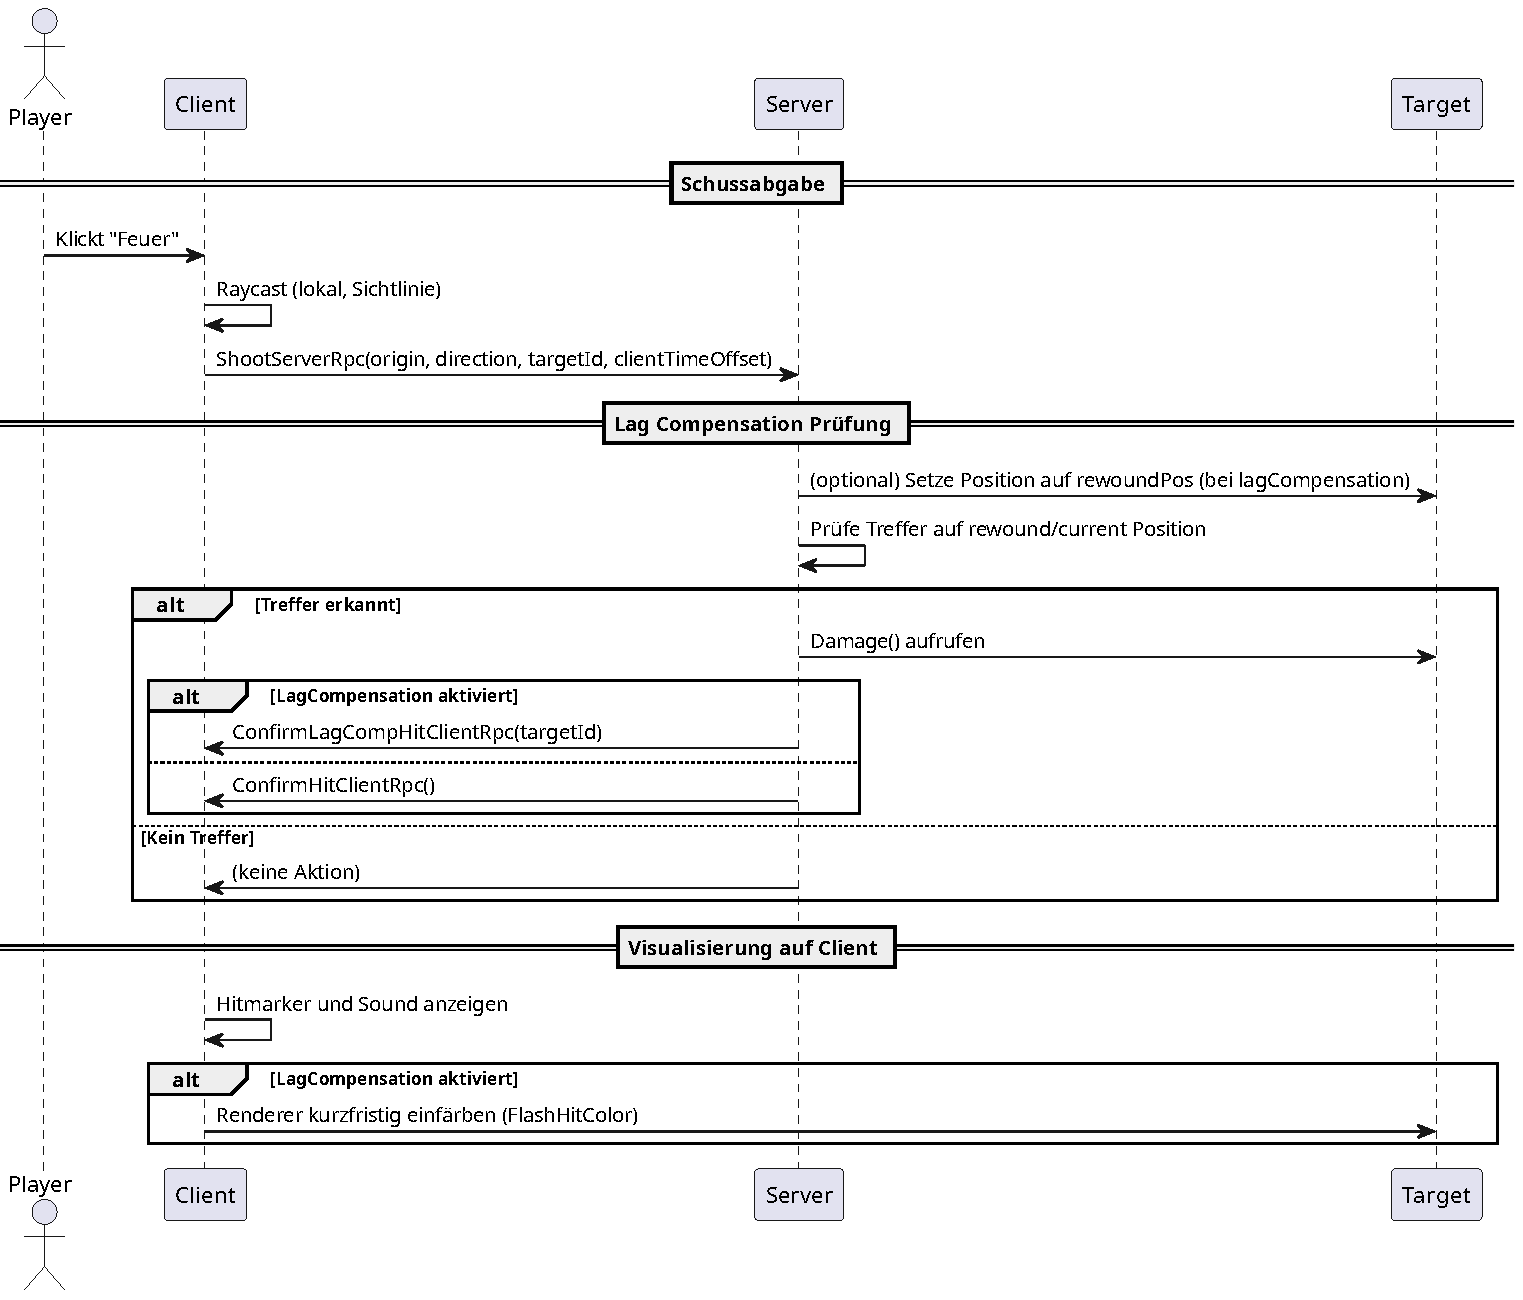
\includegraphics[width=0.9\textwidth, keepaspectratio]{out/diagrams/target-comp/target-comp.pdf} %Größe ist noch ausbaufähig...
  \caption{Visualisierung der Lag Compensation im Projekt}
  \label{fig:target-comp} %das kann man auf jeden Fall noch verbessern
\end{figure}

\newpage
Im Sequenzdiagramm \ref{fig:target-comp} ist der Ablauf der Lag-Compensation-Implementierung im Projekt dargestellt. Die Lag Compensation kann dabei gezielt aktiviert oder deaktiviert werden, um die Auswirkungen dieses Mechanismus zu untersuchen. Bei deaktivierter Lag Compensation erfolgt die Treffererkennung ausschließlich auf Basis der aktuellen Zielposition, während bei aktivierter Lag Compensation die Position des Ziels zum Schusszeitpunkt rekonstruiert und für die Trefferprüfung herangezogen wird. Dies wirkt sich nicht nur auf die Visualisierung, sondern insbesondere auf die Genauigkeit und Fairness der Treffererkennung aus. Beispielsweise wird bei aktiver Lag Compensation im Falle eines bestätigten Treffers das Zielobjekt hervorgehoben, um den Unterschied für den Spieler erkennbar zu machen.

\newpage

\section{Interpolation}
Interpolation ist in den meisten Multiplayer-Spielen unverzichtbar. Ohne sie wäre auch eine funktionierende Implementierung der Lag Compensation weitgehend wirkungslos, da die für den Client sichtbare Position des Zielobjekts keine ausreichende Aussagekraft hätte. Wenn ausschließlich zum jeweiligen Servertick eine Positionsaktualisierung an die Clients übertragen wird, kann es insbesondere bei niedrigen Tickraten zu deutlichen Ungenauigkeiten und ruckelnden Bewegungsabläufen kommen – vergleichbar mit den Effekten, die auch ohne Lag Compensation auftreten. Beispielsweise würde bei einer Tickrate von unter 10 Hz ein Spieler oder Zielobjekt nicht oft genug aktualisiert, um eine flüssige Bewegung darstellen zu können.

In den meisten modernen Spielen liegt die Tickrate allerdings deutlich höher, sodass das Fehlen von Interpolation nicht sofort als gravierendes Problem auffällt. Bei einer im Projekt verwendeten Tickrate von 60 Hz sind Unterschiede in der Bewegungsglättung für den Nutzer meist nur minimal erkennbar. Dennoch bleibt Interpolation ein wesentlicher Baustein für eine konsistente und angenehme Spielerfahrung.

Gerade im Hinblick auf Desynchronisation zwischen Server und Client spielt Interpolation eine entscheidende Rolle: Sie sorgt dafür, dass auch bei kleinen Verzögerungen oder Paketverlusten Bewegungen zwischen den übermittelten Serverpositionen sinnvoll und flüssig fortgeführt werden können. Ohne Interpolation würden solche Desynchronisationen unmittelbar als Sprünge oder Ruckler wahrgenommen werden, wohingegen eine kontinuierliche Interpolation zwischen den bekannten Zuständen die Auswirkungen von Latenz und Datenverlust für den Spieler deutlich abmildert.

Extrapolation und Interpolation ergänzen sich in modernen Multiplayer-Spielen und gelten als Gegenstücke: Während Interpolation die Bewegungen zwischen bekannten Server-Updates für den Client glättet, sorgt Extrapolation dafür, dass bei ausbleibenden Netzwerkpaketen dennoch eine plausible Fortsetzung der Bewegung berechnet wird. Bei einer durchdachten Kombination dieser beiden Verfahren bleibt der Spielfluss auch unter kritischen Netzwerkbedingungen, wie etwa hoher Latenz oder Paketverlusten, für den Spieler möglichst flüssig und konsistent.

In vielen Engines, wie beispielsweise der Source Engine von Valve, ist die Lag Compensation eng mit der Interpolationsdauer verzahnt. Der Wert der Interpolation bestimmt, wie weit die Darstellung des Spielgeschehens auf dem Client hinter den tatsächlich vom Server berechneten Zuständen zurückliegt. Eine längere Interpolationsdauer bedeutet, dass mehr verlässliche Zustände für die Glättung zur Verfügung stehen, jedoch erkauft man sich dies mit einer erhöhten „künstlichen Latenz“. Letztere bezeichnet den zusätzlichen zeitlichen Versatz, der ausschließlich durch das Interpolieren entsteht und auf den Client wirkt, unabhängig von der eigentlichen Netzwerkverbindung. 

Der Interpolationspuffer stellt eine gezielte, zusätzliche Verzögerung („künstliche Latenz“) in der Clientdarstellung dar. Diese kommt zu den eigentlichen Netzwerk- und Verarbeitungsverzögerungen hinzu und wird bewusst gewählt, um durch Interpolation stets eine ausreichend flüssige und konsistente Bewegung zwischen empfangenen Serverzuständen gewährleisten zu können Gerade in latenzkritischen Spielen ist es daher essenziell, die Interpolationsrate so niedrig wie möglich zu halten, um jede vermeidbare Quelle zusätzlicher Verzögerung zu minimieren. Gleichzeitig darf die Interpolationsdauer aber auch nicht zu gering gewählt werden, da sonst abrupte Positionssprünge oder Ruckler auftreten können, falls einzelne Serverpakete verloren gehen.

Eine adaptive Lag Compensation, die sich dynamisch an die gewählte Interpolationsdauer anpasst, kann hier Abhilfe schaffen. Sie gewährleistet, dass trotz unterschiedlich langer Pufferzeiten zwischen Server und Client eine möglichst faire und präzise Treffererkennung möglich bleibt. Insgesamt zeigt sich, dass das geschickte Zusammenspiel von Interpolation und Extrapolation – unter Berücksichtigung der mit ihnen einhergehenden Vor- und Nachteile – ein zentrales Element für eine stabile und flüssige Spielerfahrung im Online-Multiplayer darstellt~\cite{valveInterpolation}.

\newpage

\subsection{Eigenumsetzung}
Für die eigene Umsetzung dieser Mechanik ist in erster Linie nicht der Spieler an sich betroffen, wessen Positionen oder Rotationen interpoliert werden. Hierbei geht es vielmehr um das Ziel, auf welches man schießt und hängt demnach teilweise von der in \ref{custom-lag-comp} implementierten Lag Compensation zusammen.

Prinzipiell besteht in Unity die Möglichkeit, das vorhandene \texttt{NetworkTransform} entweder direkt zu verwenden oder es durch Vererbung zu erweitern und gezielt anzupassen. In beiden Fällen bleibt jedoch die umfangreiche und generische Grundstruktur der Unity-Implementierung erhalten, was zu einem gewissen Overhead und einer erhöhten Komplexität führt. Auch durch partielle Anpassungen per Vererbung kann die eigentliche Komplexität des Systems selten wesentlich reduziert werden. Für klar umrissene Anforderungen, wie sie im Rahmen dieses Projekts bestehen, ist daher eine speziell zugeschnittene Eigenimplementation oft sinnvoller, da sie sich gezielt auf die benötigten Funktionen konzentriert und unnötigen Funktionsumfang vermeidet.

Mit dieser Umsetzung können vergleichsweise wenige Einstellungen vorgenommen werden, die mit der Interpolation durch das Network Transform von Unity möglich sind. 
Hier kann dennoch die Senderate, die Verzögerung der Interpolation, das Positionslimit und die Möglichkeit die Interpolationsfunktionalität aus- oder einzuschalten.

Somit lassen sich Feinjustierungen vornehmen oder die Effekte durch Abschalten dieser Mechanik erkenntlicher machen.

\newpage

\subsection{Kernfunktion}
Die ausschlaggebende Funktion in diesem Szenario, kümmert sich um die client-seitige Interpolation und glättet somit Positions- und Rotationsdarstellung bei sich bewegenden Objekten.
\lstinputlisting[
  style=csharpStyle,
  caption={Methode \texttt{Interpolate()}},
  label={lst:Interpolation}
]{src/Interp/Interpolation.cs}

Die Methode \texttt{Interpolate(float renderTime)} sorgt dafür, dass Positions- und Rotationsänderungen eines Objekts auf dem Client auch bei unregelmäßig eintreffenden Server-Updates flüssig dargestellt werden. Zu diesem Zweck wird in einem lokalen Buffer eine Folge von Bewegungszuständen (\emph{States}) gespeichert, die jeweils einen Zeitstempel, eine Position und eine Rotation enthalten. Die Methode sucht stets die beiden States im Buffer, zwischen deren Zeitstempeln der gewünschte Anzeigemoment (\texttt{renderTime}) liegt. Mit Hilfe eines Interpolationsfaktors wird dann eine Position und Rotation berechnet, die zeitlich genau zwischen diesen beiden Punkten liegt. So entsteht für den Spieler der Eindruck einer kontinuierlichen Bewegung, selbst wenn neue Bewegungsdaten nur in größeren Abständen eintreffen. Sollte keine Interpolation möglich sein, etwa weil zu wenige States vorliegen, wird stattdessen einfach der letzte bekannte Zustand übernommen.

\dots